\documentclass[12pt,a4paper]{article}
\usepackage[utf8]{inputenc}
\usepackage[russian]{babel}
\usepackage[OT1]{fontenc}
\usepackage{graphicx}
\usepackage{calc}
\usepackage[margin=15mm]{geometry}
% счётчик задач
\newcounter{notask}
\setcounter{notask}{1}

% условие без картинки
\newcommand{\task}[2]{
\hrule
\hbox to \textwidth {%
     \vrule
\parbox[t]{0.04\textwidth}{\smallskip \centering #1}%
     \vrule%
\hfill%
     \parbox[t]{0.93\textwidth}{\smallskip #2 \smallskip}\hfill%
\vrule
}
\hrule
    \addtocounter{notask}{1}
    \pagebreak[2]
}

\newlength{\h}
\newsavebox{\taskbox}
\newlength{\x}
\newsavebox{\pictbox}

% условие с картинкой (картинка выравнивается по центру)
\newcommand{\taskpic}[3]{
\savebox{\taskbox}{\parbox[t]{0.93\textwidth-4.3cm}{\smallskip #2 \smallskip}}
\savebox{\pictbox}{\parbox[t]{4cm}{\smallskip \centering
     \vspace{0pt} #3 \smallskip}}
\h=\ht\taskbox
\advance\h\dp\taskbox
\x=\ht\pictbox
\advance\x\dp\pictbox
\hrule
\hbox to \textwidth {%
\vrule\parbox[t][\maxof{\h}{\x}][t]{0.04\textwidth}{ \smallskip
     \centering #1 }\vrule%
\hfill\parbox[t][\maxof{\h}{\x}][t]{0.93\textwidth-4.3cm}{\smallskip #2
     \smallskip}\hfill\vrule%
\hfill\parbox[t][\maxof{\h}{\x}][c]{4cm}{\hfil #3 \hfil}\hfill\vrule
}
\hrule
\addtocounter{notask}{1}
\pagebreak[2]
}
\pagestyle{empty}


\begin{document}
\begin{center}
\begin{Large}
\textsc{ГЦФО. 9 класс. 2014/15.}
\end{Large}
\end{center}
\taskpic{1}{В вагоне, движущемся равноускоренно по прямым горизонтальным рельсам, экспериментатор фотографировал упругий шарик, отскакивающий от пола. При этом он отпускал шарик без начальной скорости (относительно вагона) с некоторой фиксированной высоты. Фотоаппарат был неподвижен относительно вагона, плоскость траектории шарика лежала в плоскости снимка. В результате экспериментатор получил изображение траектории шарика между первым и вторым отскоками (см. рис.). Найдите ускорение вагона. Чему равно расстояние между первой и второй точками касания шариками пола, если время между отскоками равно $\tau=0{,}4$~с? Постоянная $g=9{,}8$~м/с$^2$.}{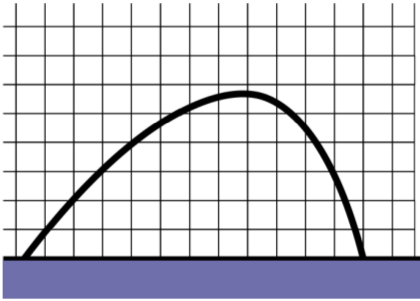
\includegraphics[width=4cm]{1}}
\taskpic{5}{В солдата, сидящего в окопе, неприятель выстрелил из мортиры (см. рис.). Снаряд летел ровно на него, но до окопа не долетел. С точки зрения солдата снаряд поднимался в течение $t_1$ секунд, а опускался быстрее, за $t_2$ секунд, смотрел он из окопа от уровня земли. Известно, что неприятельские мортиры стреляют под углом $\alpha$ к горизонту, а модуль начальной скорости снаряда равен $V_0$. Найдите, на каком расстоянии от окопа упал снаряд. Сопротивлением воздуха пренебречь, ускорение свободного падения равно $g$.}{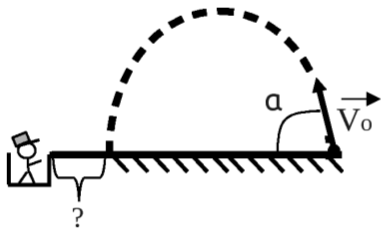
\includegraphics[width=4cm]{5}}
\taskpic{6}{Наклонная плоскость образует угол $\alpha$ с горизонтом. С высоты $H$ на нее падает мячик. Считая удары мячика о плоскость абсолютно упругими, определите расстояние между точками $n$-го и $(n+1)$-го отскока мячика от плоскости.}{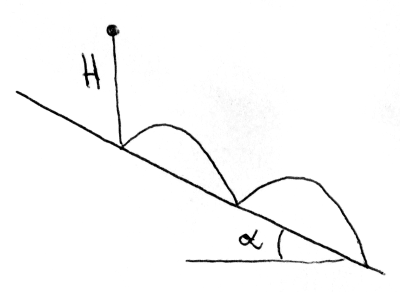
\includegraphics[width=3cm]{6}}
\taskpic{7}{Тело соскальзывает с гладкой горки с высоты $H$. Отрыв тела от горки происходит на высоте $h$, при этом скорость тела горизонтальна. При каком значении $h$ дальность полета тела будет максимальной?}{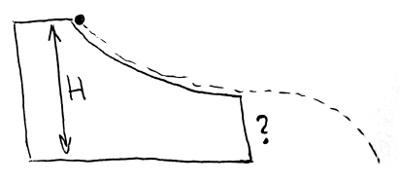
\includegraphics[width=4cm]{7}}
\taskpic{8}{Для создания зловещего механизма Мегамозг вскрыл тайное хранилище, содержащее три резистора с сопротивлениями 1~Ом, 4~Ом и 5~Ом. Однако из-за происков врагов надписи на резисторах оказались стерты. Тогда Мегамозг собрал из них верхнюю схему, изображенную на рисунке, и подключил к ней батарейку напряжением 1,2~B. Амперметр показал ток 0,5~А. Затем он собрал нижнюю схему, и, когда он подключил эту схему к батарейке, амперметр сгорел. Однако мастер злодейства не расстроился, ведь теперь он знал, где какое сопротивление. Чему равны сопротивления $R_1$, $R_2$, $R_3$? Амперметр сгорает, если через него течет ток больше 1~А.}{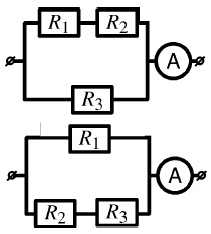
\includegraphics[width=4cm]{8}}
\taskpic{9}{Две прямые, пересекающиеся под углом $\alpha$, движутся перпендикулярно самим себе со скоростями $v_1$ и $v_2$.  Определите скорость $v$ точки пересечения прямых}{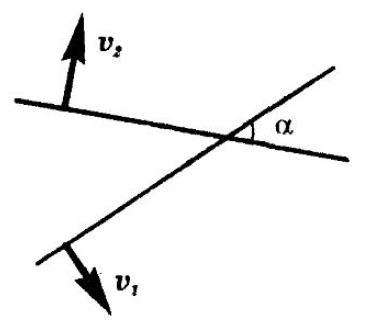
\includegraphics[width=3cm]{9}}

\end{document}